\section{Refreshers}

\subsection{Crypto Refresher}

\subsubsection{Definitions}

\begin{itemize}
    \item \textbf{Secrecy:} Keep data hidden from unintended receivers.
    
    \item \textbf{Confidentiality:} Keep someone else's data secret.
    
    \item \textbf{Privacy:} Keep data about a person secret.
    
    \item \textbf{Anonymity:} Keep identity of a protocol participant secret.
    
    \item \textbf{Data Integrity:} Ensure data is correct (no unauthorized / improper changes).
    
    \item \textbf{Entity Authentication/Identification:} Verify the identity of another protocol participant.
    
    \item \textbf{Data Authentication:} Ensure that data originates from claimed sender.
\end{itemize}

\subsubsection{Symmetric Cryptography (Shared/Same-Key)}

\begin{figure}[h]
	\centering
	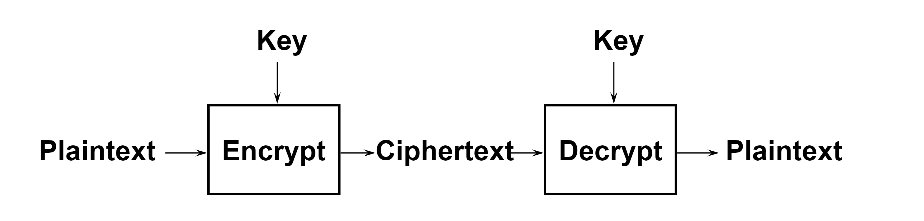
\includegraphics[scale=0.5]{images/1-symm_crypto.PNG}
	\caption{Symmetric encryption primitives.}
	\label{fig:sym_crypto}
\end{figure}

For a plaintext enrypted with key $K$, we write \{plaintext\}$_K$. The main challenge of symmetric cryptography is the distribution of the secret key (a confidential and authentic channel is required).

\paragraph{Stream / State Ciphers}
Plaintext digits combined with a pseudorandom cipher digit stream (keystream) to encrypt them one at a time with the corresponding keystream digit (typically with an XOR operation).

\paragraph{Keystream}
Utilize a pseudorandom generator (PRG) to generate a keystream from a seed.
E.g. Use shared key $k$ and initialization vector $IV$ for the seed, share cipher text and $IV$ (ciphertext = plaintext $\oplus$ PRG($k, IV$).

\paragraph{Initialization Vector / Nonce}
Pseudorandom fixed-size input to a cryptographic primitive. Best if non-repeating in repeated encryption applications.

\paragraph{One-Time Pad Stream Cipher}
Plaintext encryption using a one-time pre-shared key with the same size (or longer than) the message being sent. Impossible to break if: 1) key is truly random and 2) key is never (partially) reused.

\paragraph{ChaCha / Salsa Stream Cipher}
A 512-bit keystream is generated with a 256-bit key and a 64-bit nonce using add-rotate-XOR operations. %TODO: more on this?

\paragraph{Keystream Reuse Attack}
If $A$ and $B$ are same-length plaintexts encrypted with the same key $K$, we have (with $C$ being the key stream):

$$
\{A\}_K = A \oplus C \text{ and } \{B\}_K = B \oplus C
$$

$$
\{A\}_K \oplus \{B\}_K = (A \oplus C) \oplus (B \oplus C) = A \oplus B \oplus C \oplus C = A \oplus B
$$

Even without knowing $A$ or $B$ specifically, both plaintexts can be easily derived / analyzed.

\paragraph{Ciphertext Modification Attack}
Changing digits of the ciphertext will alter the corresponding values in the plaintext after decryption. Authenticity of ciphertext is required to defend against this attack.

\paragraph{Block Ciphers}
Blocks (fixed-length groups of bits, last block padding if needed) are encrypted using a symmetric key each (one-to-one mapping).
E.g. Advanced Encryption Standard (AES).

\paragraph{Mode of Operation}
Describes how to repeatedly apply a cipher's single-block operation to encrypt the data. There are two categories: confidentiality-only (ECB, CBC, CTR, etc.) and authenticated encryption (AE) that combines confidentiality and authenticity. Integrity protection is an entirely separate goal seen in AEAD only.

\paragraph{Electronic Code Book (ECB)} 
Natural approach - split plaintext into blocks and use the same key for each block. Has the disadvantage that equal blocks correspond to equal ciphertexts - lack of diffusion. ECB does not hide data patterns well (esp. in images with large areas of uniform colors).

\paragraph{Cipher Block Chaining (CBC)}
Apply XOR to each block with previous ciphertext before encrypting. Use an $IV$ for the first block. Each ciphertext block depends on all plaintext blocks processed up to that point. Cannot be parallelized and message must be padded to a multiple of cipher block size. Plaintext block can be recovered from two adjacent blocks of ciphertext (allows for parallelized decryption).

\paragraph{Counter Mode (CTR)}
Turn block cipher into a stream cipher. Generates the next keystream block by encrypting successive values of a counter (any function that does not repeat for a long time, e.g. increment by one counter). Use an $IV$ for the first block and increment for next blocks. Has the same vulnerabilities as any other stream cipher.

\paragraph{Authenticated Encryption}
Ensures confidentiality and authenticity of data.
E.g. Encrypt-then-MAC (EtM), Encrypt-and-MAC (E\&M), MAC-then-Encrypt (MtE).

\paragraph{Message Authentication Code (MAC)}
Cryptographic checksum for message authentication and integrity. Can only be calculated with a shared secret key (MAC$_K$(M)).

\begin{figure}[h]
	\centering
	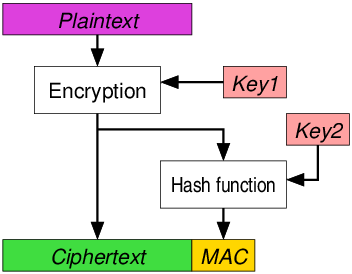
\includegraphics[scale=0.4]{images/1-EtM.png}
	\caption{EtM approach.}
	\label{fig:etm}
\end{figure}

\begin{figure}[h]
	\centering
	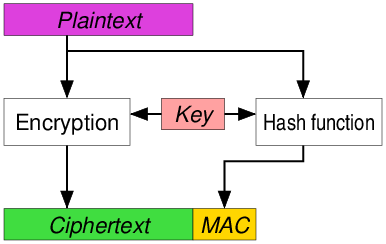
\includegraphics[scale=0.4]{images/1-EaM.png}
	\caption{E\&M approach.}
	\label{fig:eam}
\end{figure}

\begin{figure}[h]
	\centering
	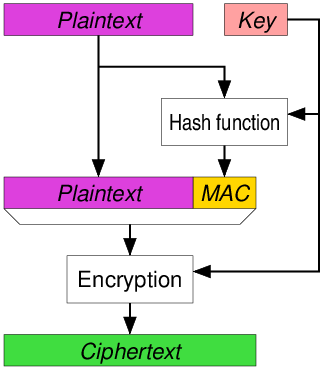
\includegraphics[scale=0.4]{images/1-MtE.png}
	\caption{MtE approach.}
	\label{fig:mte}
\end{figure}

\paragraph{Authenticated Encryption with Associated Data (AEAD)}
Allows a recipient to check the integrity of both the encrypted and unecrypted message (on top of confidentiality and authorization). Based on Encrypt-and-MAC (E\&M).

\paragraph{Galois Counter Mode (GCM)}
AEAD based on a block cipher in CTR mode (block size of 128 bits) and Galois MAC - mostly used with AES (AES-GCM). 

\begin{figure}[h]
	\centering
	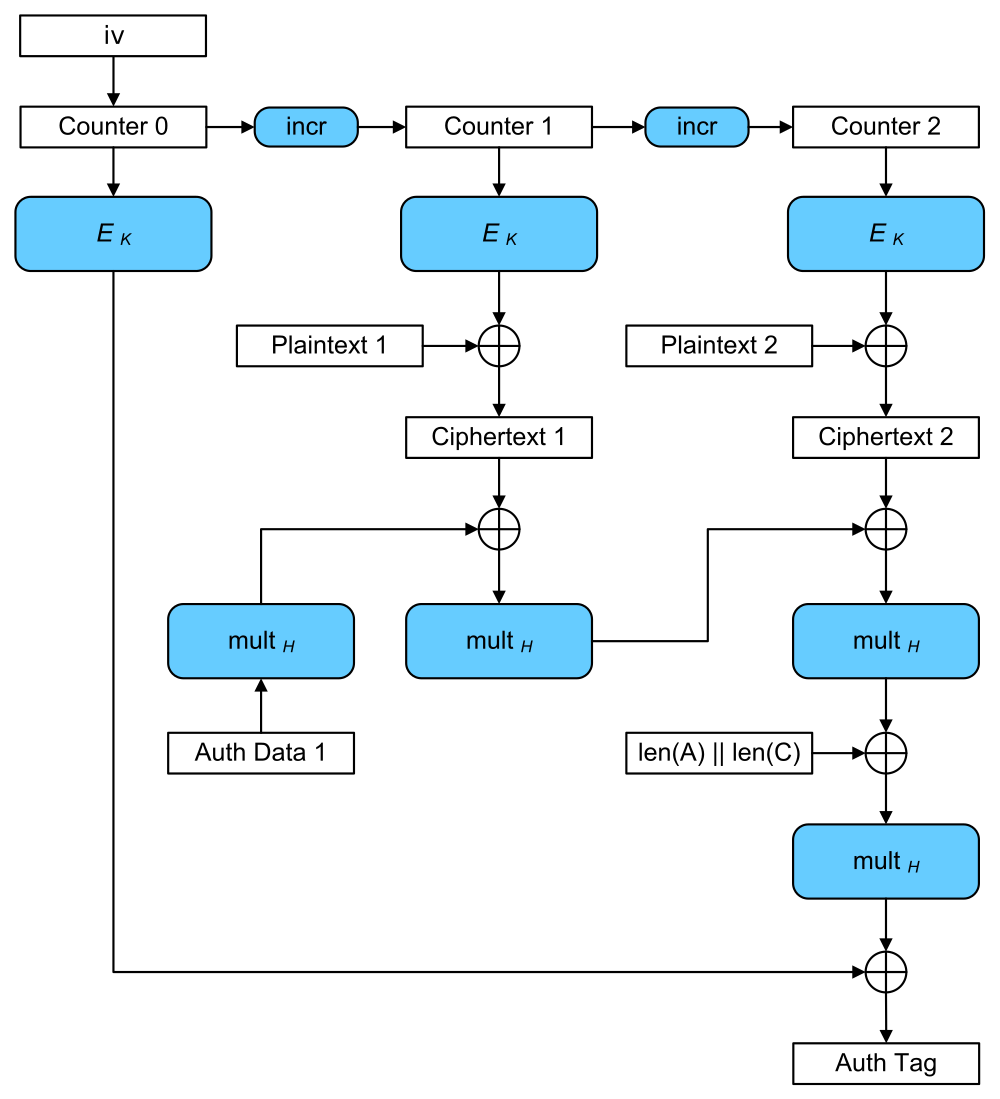
\includegraphics[scale=0.2]{images/1-gcm.png}
	\caption{GCM with only two plaintexts.}
	\label{fig:gcm}
\end{figure}


\subsubsection{Asymmetric / Public-Key Cryptography / PKI}

%TODO examples of key exchange

Cryptographic primitives using pairs of keys (public and private). The pairs are generated using cryptographic one-way functions. Can be used to establish a secret symmetric key.

Messages are encrypted using the receiver's public key and can only be decrypted with the receiver's private key. To ensure authenticity, a message can additionally be signed with the sender's private key and verified with their public key.

The main challenge is the authentication of the key (an authentic channel is required).

\paragraph{Diffie-Hellman Key Exchange}
A method to securely exchange a key over a public channel based on the discrete logarithm problem (see Figure \ref{fig:dhke}). Is susceptible to man-in-the-middle attacks in which attacker impersonates either receiver to each sender, resulting in two different established keys.

\begin{figure}[h]
	\centering
	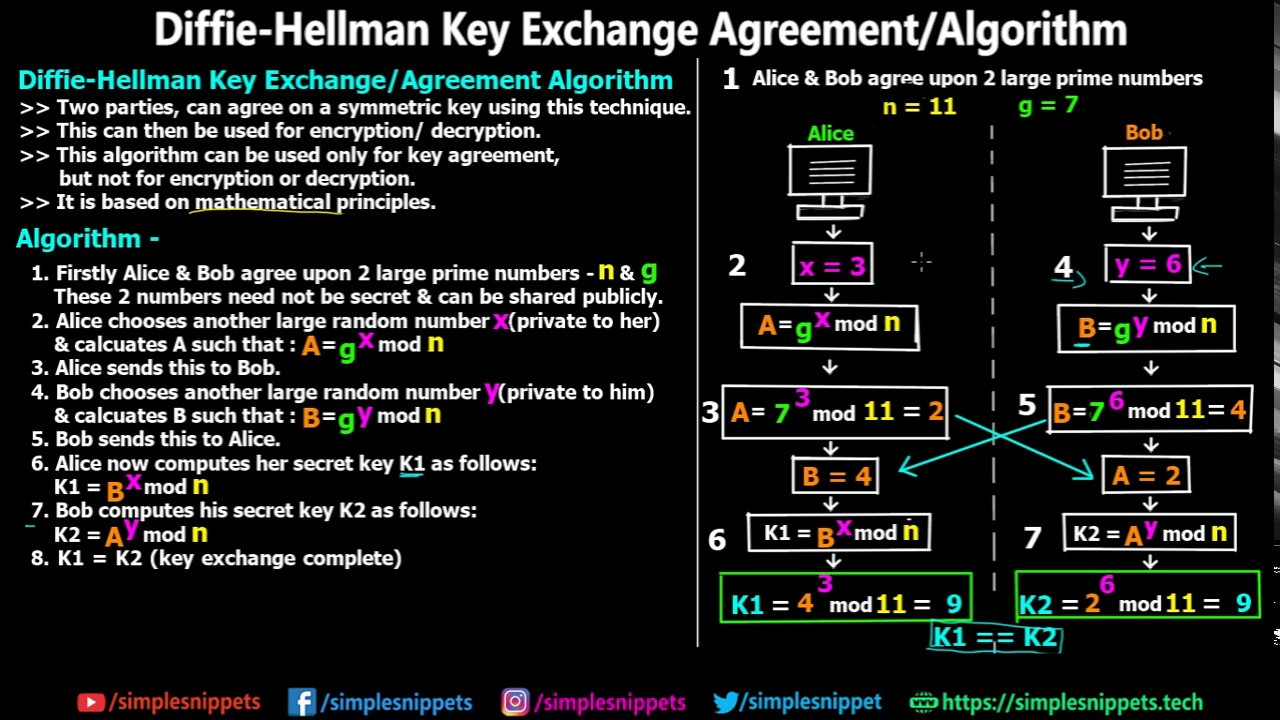
\includegraphics[scale=0.2]{images/1-diffie_hellman.jpg}
	\caption{Diffie-Hellman key exchange.}
	\label{fig:dhke}
\end{figure}

\paragraph{Discrete Logarithm Problem}
Given $x$, $g$ and $p$ find $a$ ($g^a$ mod $p = x$).

\paragraph{RSA Algorithm} Same as with Diffie-Hellman, just in a different way (see Figure \ref{fig:rsa}).

\begin{figure}[h]
	\centering
	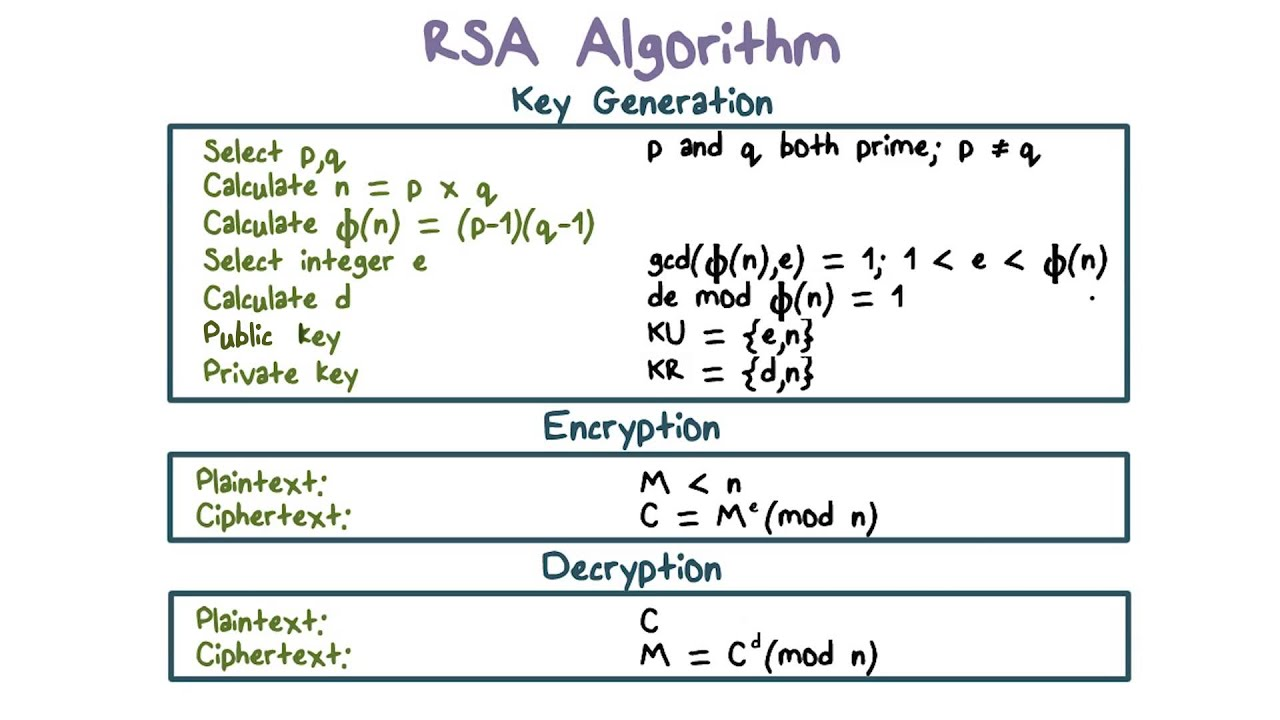
\includegraphics[scale=0.2]{images/1-rsa.jpg}
	\caption{RSA key generation and de/encryption.}
	\label{fig:rsa}
\end{figure}

\paragraph{Encrypted Key Exchange (EKE)}
Both ends share a password $P$ and want to authenticate each other along with establishing a shared secret key (see Figure \ref{fig:dh_eke}).

\begin{figure}[h]
	\centering
	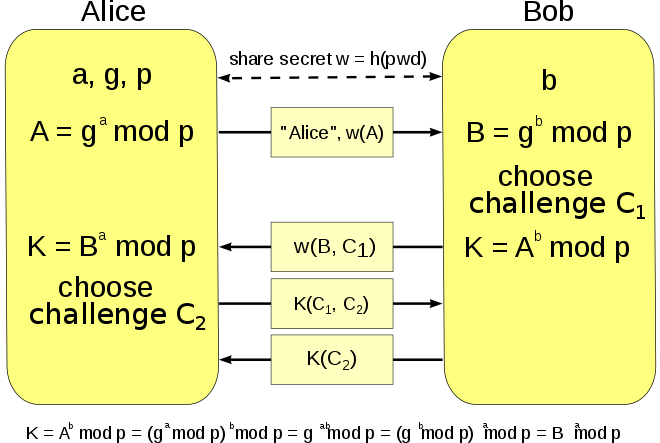
\includegraphics[scale=0.3]{images/1-dh_eke.png}
	\caption{DH-EKE scheme.}
	\label{fig:dh_eke}
\end{figure}

\paragraph{Authentication vs. Signature}
Authentication enables a receiver to verify the origin of a message, but it cannot convince a third party of the origin. A signature allows for the verification of origin and will convince a third party of it as well (a signature provides authentication).

\subsubsection{Hash Functions}

\paragraph{Cryptographic Hash Functions}
Map an arbitrary-length input into a finite length output with the following properties:

\begin{itemize}
    \item \textbf{One-way:} given $y = H(x)$, one cannot find $x'$ s.t. $H(x') = y$.
    \item \textbf{Weak collision resistance:} given $x$, one cannot find $x' \neq x$ s.t. $H(x) = H(x')$.
    \item \textbf{Strong collision resistance:} one cannot find $x' \neq x$ s.t. $H(x) = H(x')$.
\end{itemize}

They can be used for digital signatures, MACs and other forms of authentication. Also used for fingerprinting (unique IDs, no duplicates) and as checksums (check integrity). Most common cryptographic hash functions include MD5, SHA-1, SHA-2 and SHA-3.

SHA-1 is known for collision attacks. E.g. Git only uses SHA-1 value to identify commits - attacker can commit good code and distribute a repo version with bad code that has the same SHA-1 value.

%TODO add exercise 2.8 - calculation with hash collisions

\paragraph{One-Way Hash Chain}
A method to produce many one-time keys from a single key. Pick a random starting value and a public one-way hash function, continuously apply function to resulting values and use results in reverse order of construction. Allows for authentication of $r_i$ using $r_j$ where $j < i$ and $r_j = F(r_i)$.

\paragraph{Merkle Hash Trees (Binary Hash Chain)}
Efficient and secure verification of large data. Data is divided into blocks with each block labelled with its cryptographic hash value (leaf nodes). Every non-leaf node is the hash value of the concatenated hash values of its two children (if binary). To demonstrate that a leaf node is part of a binary tree, it is required to compute a number of hashes proportional to the log of leaf nodes - this allows for partial checking (as compared to hash lists where we would need the full file). Usually, the root hash received from a trusted source is compared to a hash tree from a potentially untrusted source.




%TODO: conversions and useful units





\subsection{Network Refresher}
%TODO esp. NAT, BGP, DNS

